\documentclass{beamer}

%\usetheme{Goettingen}
%\usetheme{Berkeley}
%\usetheme{Boadilla}
%\usetheme{Copenhagen}

\usepackage[math]{iwona}
\usepackage{graphicx}
\usepackage{wrapfig}
\usepackage{pgf,tikz}
\usetikzlibrary{shapes.gates.logic.US,trees,positioning,arrows}
\usepackage{hyperref}
\hypersetup{colorlinks=true}

\usepackage[utf8]{inputenc}
\usepackage[spanish]{babel}


\title[Taller de \LaTeX]{Taller de gr\'aficos con \LaTeX}
\author[Los presentes]{Orientamat}
\institute[UGR]{Universidad de Granada}
\date{21 de Marzo de 2014}
\begin{document}

\maketitle

\section{Formatos gr\'aficos}
\begin{frame}{Generalidades sobre formatos gr\'aficos}
\begin{block}{Mapas de bits} 
\begin{center}
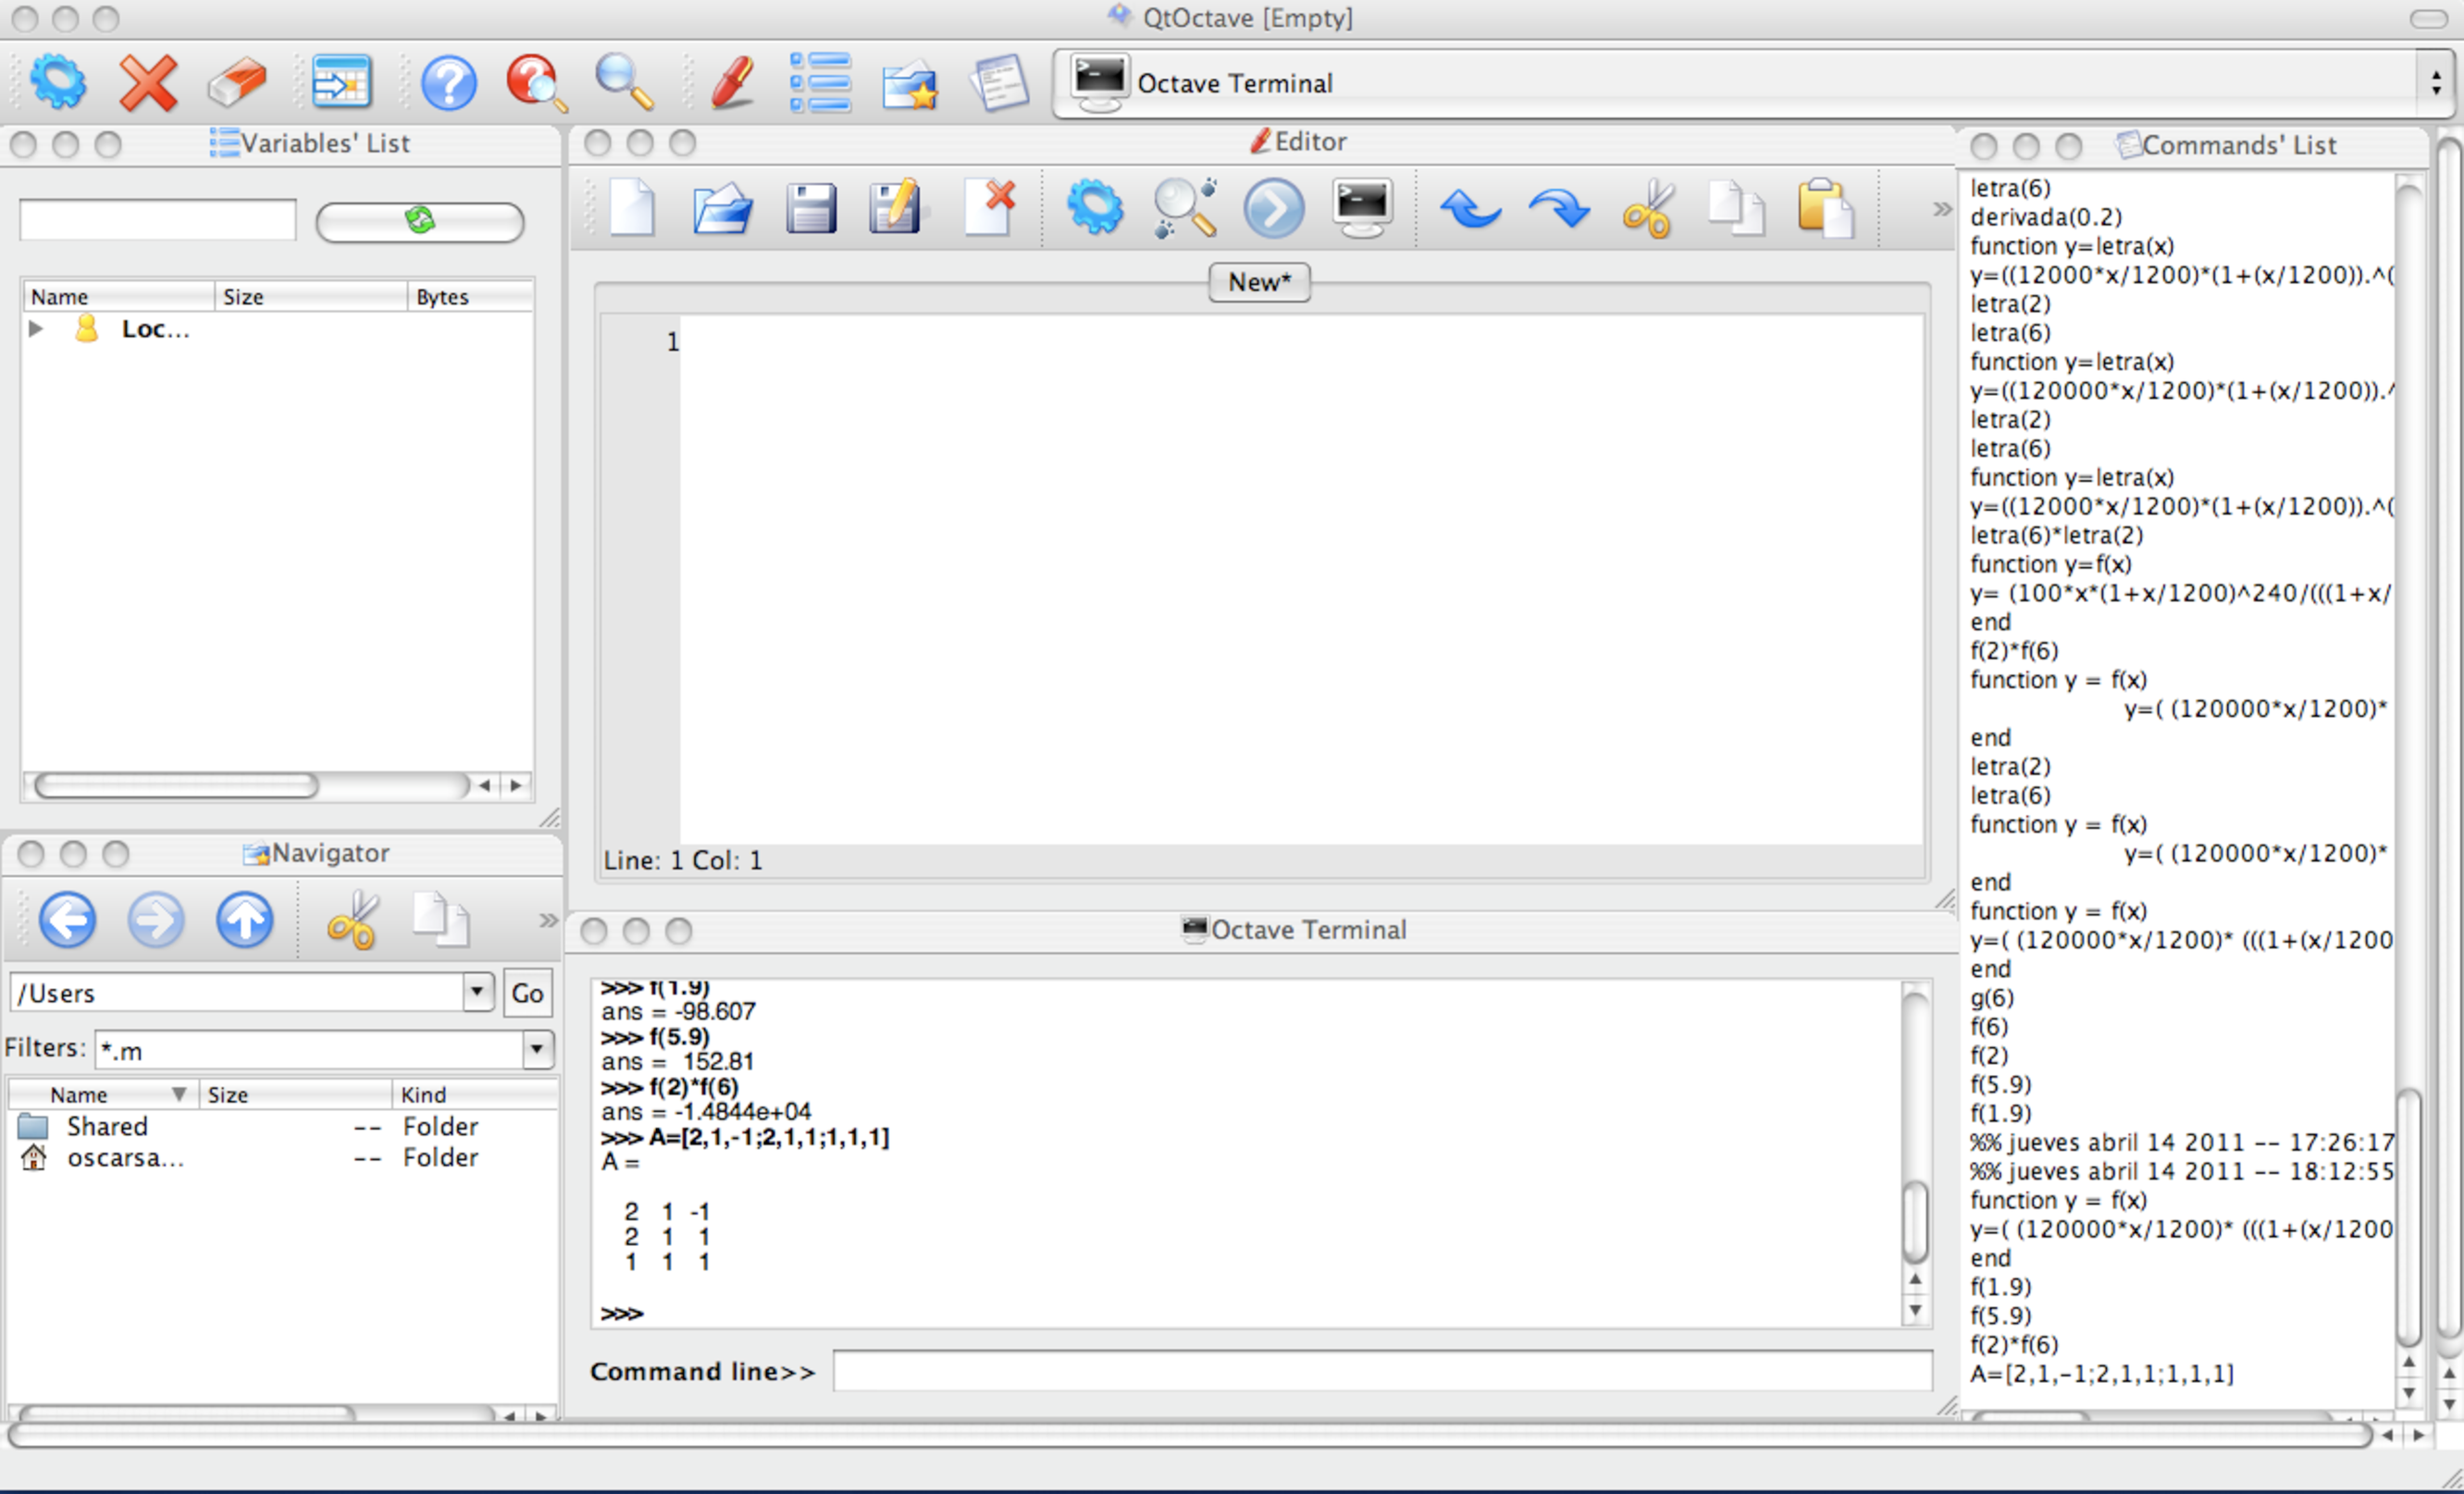
\includegraphics[width=7cm]{./graficos/QtOctave.pdf}
\end{center}
Extensiones: BMP, JPEG, GIF, PNG y TIFF. \\
{\small Desventaja: deformaciones al reescalar y gran tama\~no.}
\end{block}
\end{frame}
\begin{frame}
\begin{block} {Gr\'aficos vectoriales} 
\begin{center}
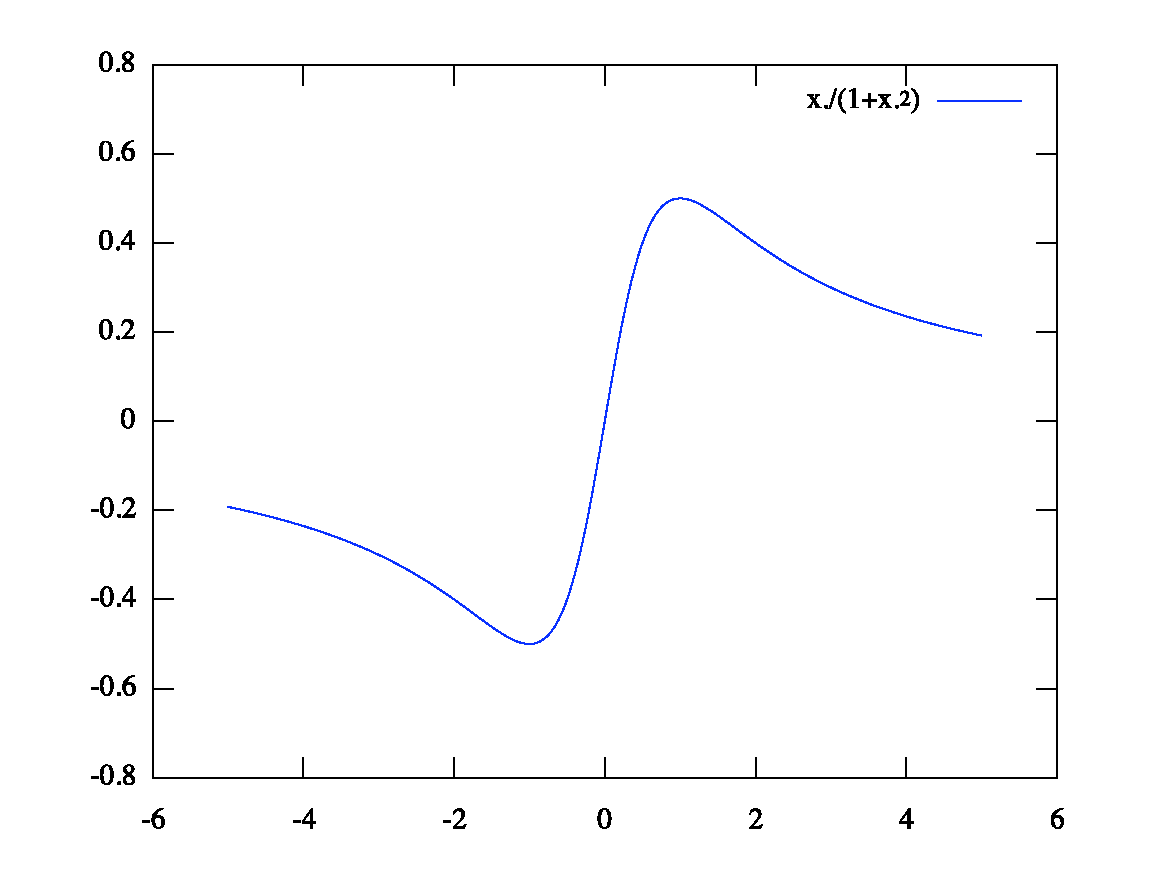
\includegraphics[width=7cm]{graficos/fplot.pdf}
\end{center}
Extensiones: EPS, PDF, SVG, WMF \\
{\small Nota: !`Estos archivos pueden insertar mapas de bits! }
\end{block}
\end{frame}

%%%%%%%%%%%%%%%%%%%%%%%%%%%%%%%%%%%%%%%%

\begin{frame}{Preparaci\'on de gr\'aficos para insertar en \LaTeX}
El formato del gr\'afico a insertar depende del compilador empleado:
\begin{enumerate}
\item \it{latex + dvips}  se requiere PS / EPS {\scriptsize(con \href{http://tex.stackexchange.com/questions/133786/no-boundingbox-error-message}{BoundingBox})}
\item \it {pdflatex} se requiere PNG {\scriptsize(mapas de bits simples)}, JPEG {\scriptsize(fotograf\'ias)} o PDF {\scriptsize(gr\'aficos vectoriales)}
\end{enumerate}

\vspace{0.5cm}
Esto requiere de programas espec\'ificos de transformaci\'on:
\begin{itemize}
\item {\sc EPS a PDF}: \href{http://tug.org/epstopdf/}{epstopdf}
%\item {\sc JPEG a EPS}: \href{http://www.pdflib.com/download/free-software/jpeg2ps/}{jpeg2ps}
\item {\sc Todo a Todo}: \href{http://www.inkscape.org/es/}{Inkscape}, 
\href{http://www.imagemagick.org}{ImageMagick} o \href{http://www.gimp.org/}{Gimp}
\item ........
\end{itemize}
Nosotros nos centramos en c\'omo generar gr\'aficos con programas de matem\'aticas.
\end{frame}
%%%%%%%%%%%%%%%%%%%%%%%%%%%%%%%%%%%%%%%%%%
\section{Inserci\'on de un gr\'afico}
\begin{frame}[fragile]{Insertar el gr\'afico como una figura}
Declaraci\'on del paquete graphicx en el pre\'ambulo:
\begin{verbatim}\usepackage{graphicx} \end{verbatim}

Inserci\'on del gr\'afico en el documento:
\begin{verbatim}
\begin{figure}
  \centering
  \includegraphics[parametros]{nombregrafico}
  \caption{Leyenda bajo el grafico}
  \label{fig:etiqueta}
\end{figure}
\end{verbatim}
Mediante los par\'ametros se puede modificar el aspecto:\\
\begin{verbatim}height=0.5\textwidth, keepaspectratio,angle=90, ....\end{verbatim}
Para profundizar ver \cite{ManualImportingGraphics,ManualLatexWikilibros} .
\end{frame}
%%%%%%%%%%%%%%%%%%%%%%%%%%%%%%%%%%%%%%%%%%%%
\begin{frame}[fragile]
\begin{exampleblock}{Ejercicio 1: Inserci\'on de un gr\'afico creado con Octave}
{\small As\'i el comando
\\%%
\verb|>> t = 0:0.2:6.3;  plot (t, sin(t),'-@r*;sin(t);')|
%\\%%
%\verb|>> t = 0:0.2:6.3; plot (t, sin(t),'@gx','markersize',3)|\\
representa la funci\'on seno variando dichas propiedades.
\begin{figure}
\begin{center}
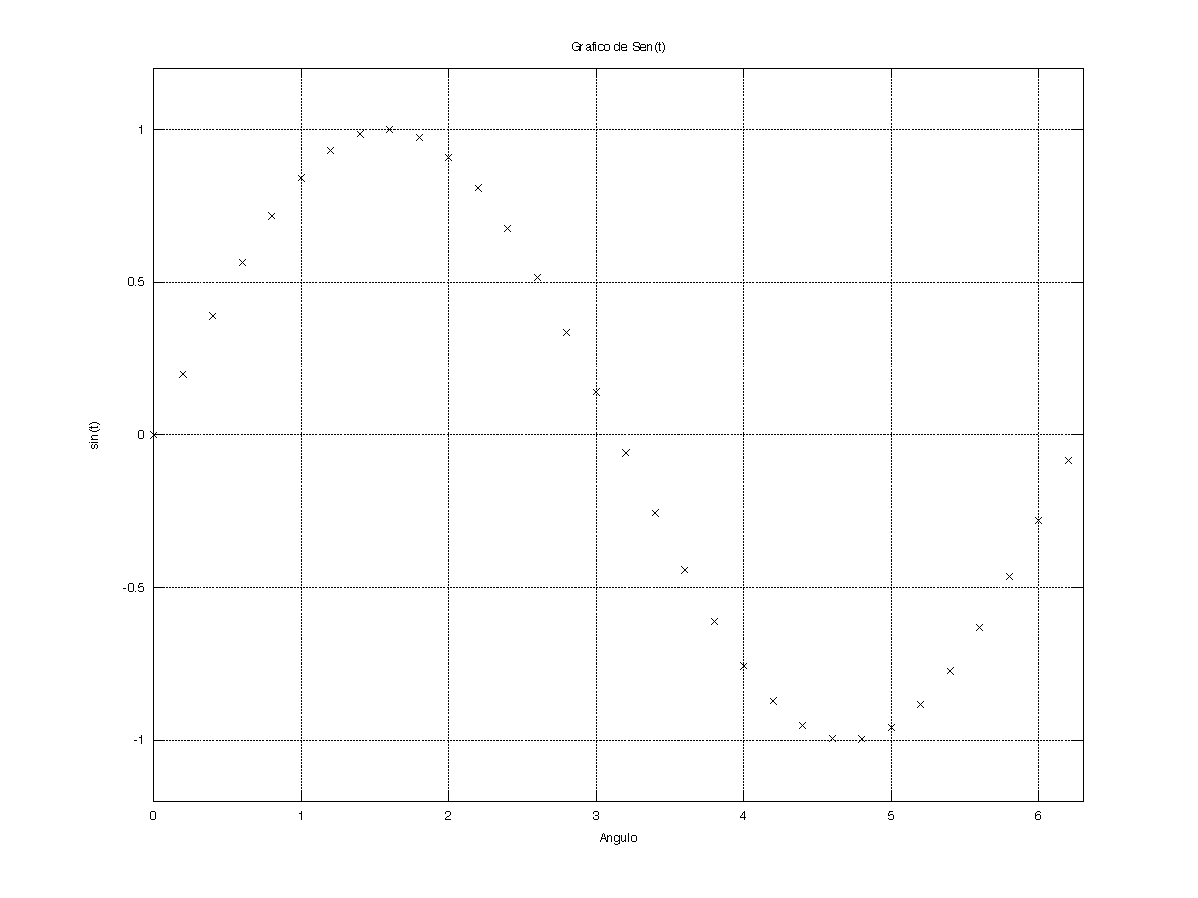
\includegraphics[width=0.35\textwidth]{graficos/sin.pdf}
\end{center}
\caption{Gr\'afico con estilo \label{figura:sinestilo}
}
\end{figure}
%\begin{wrapfigure}{r}{0.4\textwidth}
%  \begin{center}
%  %  \vspace{-20pt}
%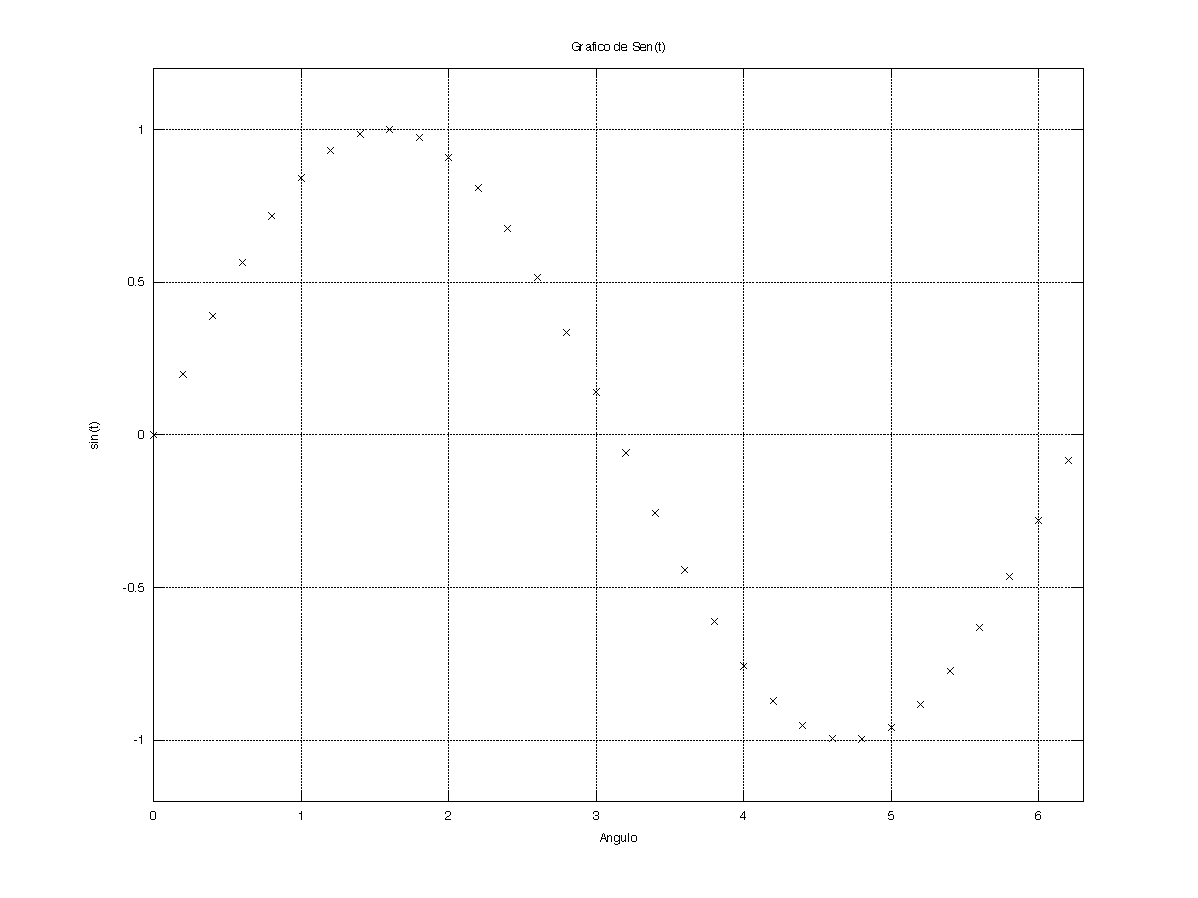
\includegraphics[width=5cm]{graficos/sin.pdf}
%  \end{center}
% \vspace{-30pt}
%  \caption{Gr\'afico con estilo \label{figura:sinestilo}
%}
%\end{wrapfigure}
%Una vez generado el gr\'afico, se pueden a\~nadir t\'itulos, etiquetas a los ejes, mallados o incluso redimensionar la figura
%tal y como indican los siguientes comandos:
%\\%%
%\verb|>> title('Grafico de Sen(t)')|
%\\%%
%\verb|>> xlabel('Angulo')|
%\\%%
%\verb|>> ylabel('sin(t)')|
%\\%%
%\verb|>> grid on|
%\\%%
%\verb|>> axis([0 6.3 -1.2 1.2])|
%\\
%donde el comando \it{axis} requiere como argumento un vector definido como $(x_{min},x_{max},y_{min},y_{max})$
Para guardar un gr\'afico en formatos EPS o PDF se puede emplear el comando print de la siguiente manera:
\\
\verb|>> print('grafico1.eps','-deps')| \\
\verb|>> print('grafico1.pdf','-dpdf')| \\
dango lugar al gr\'afico que presentamos en la figura \ref{figura:sinestilo}.
}
\end{exampleblock}
\end{frame}

%%%%%%%%%%%%%%%%%%%%%%%%%%%%%%%%%%%%%%%%%%
\begin{frame}[fragile]{El paquete wrapfig}
El paquete  \href{http://www.ctan.org/pkg/wrapfig}{wrapfig} permite integrar el gr\'afico con el texto.
\vskip 12pt
Declaraci\'on del paquete wrapfig en el pre\'ambulo:
\begin{verbatim} \usepackage{wrapfig} \end{verbatim}

Inserci\'on del gr\'afico en el documento:
\begin{verbatim}
\begin{wrapfigure}{r}{<width>}
  \includegraphics[parametros]{nombregrafico}
  \caption{Leyenda bajo el grafico}
  \label{fig:etiqueta}
\end{wrapfigure}
\end{verbatim}

%Para profundizar ver \cite{wrapfigure} .
\end{frame}


%%%%%%%%%%%%%%%%%%%%%%%%%%%%%%%%%%%%%%%%%%%%
\begin{frame}[fragile]
\begin{exampleblock}{Ejercicio 2: Inserci\'on de un gr\'afico con wrapfigure}
{\small As\'i el comando
\\%%
\verb|>> t = 0:0.2:6.3;  plot (t, sin(t),'-@r*;sin(t);')|
representa la funci\'on seno variando dichas propiedades.
Una vez generado el gr\'afico, se pueden a\~nadir t\'itulos, etiquetas a los ejes, mallados o incluso redimensionar la figura
tal y como indican los siguientes comandos:\\%%
\begin{wrapfigure}{r}{0.5\textwidth}
\begin{center}
\vspace{-30pt}
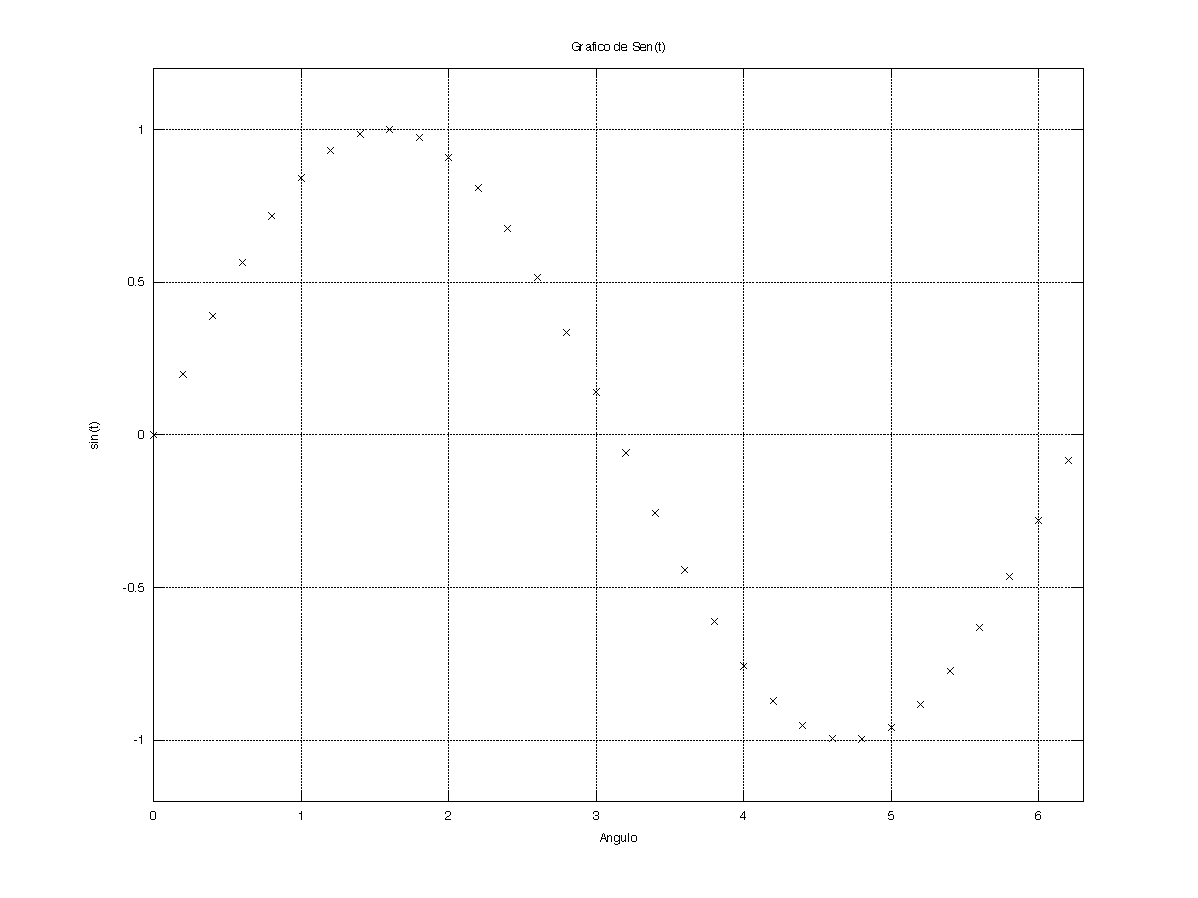
\includegraphics[width=5cm]{graficos/sin.pdf}
  \end{center}
\vspace{-25pt}
  \caption{{\tiny Gr\'afico con estilo \label{figura:sinestilo1}}}
\end{wrapfigure}
\verb|>> title('Grafico de Sen(t)')|
\\%%
\verb|>> xlabel('Angulo')|
\\%%
\verb|>> ylabel('sin(t)')|
\\%%
\verb|>> grid on|
\\%%

Para guardar un gr\'afico en formatos EPS o PDF se puede emplear el comando print de la siguiente manera:
\\
\verb|>> print('grafico1.eps','-deps')| \\
\verb|>> print('grafico1.pdf ','-dpdf')| \\
dango lugar al gr\'afico que presentamos en la fig. \ref{figura:sinestilo1}.
}
\end{exampleblock}
\end{frame}

%%%%%%%%%%%%%%%%%%%%%%%%%%%%%%%%%%%%%%%%%%%%%%%%%%%%
\begin{frame}[fragile]
\begin{exampleblock}{Ejercicio 3: Inserci\'on de varios gr\'aficos}
\begin{figure}
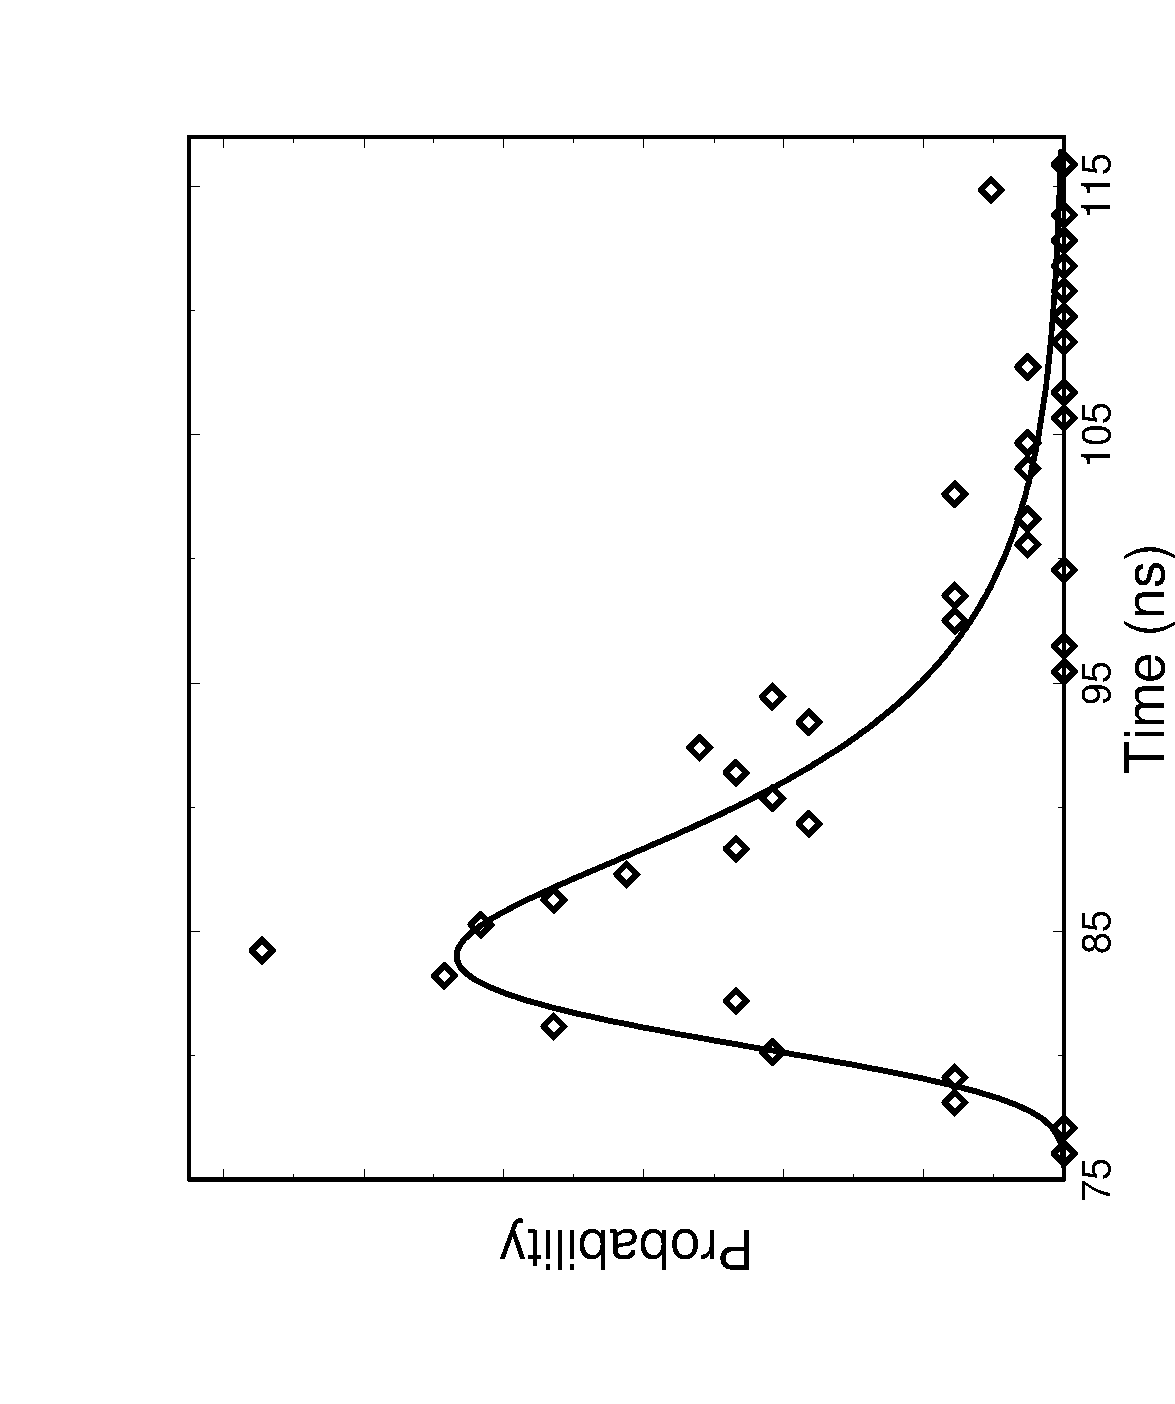
\includegraphics[angle=270, width=4cm]{./graficos/fig_9.pdf}
\hspace{1cm}
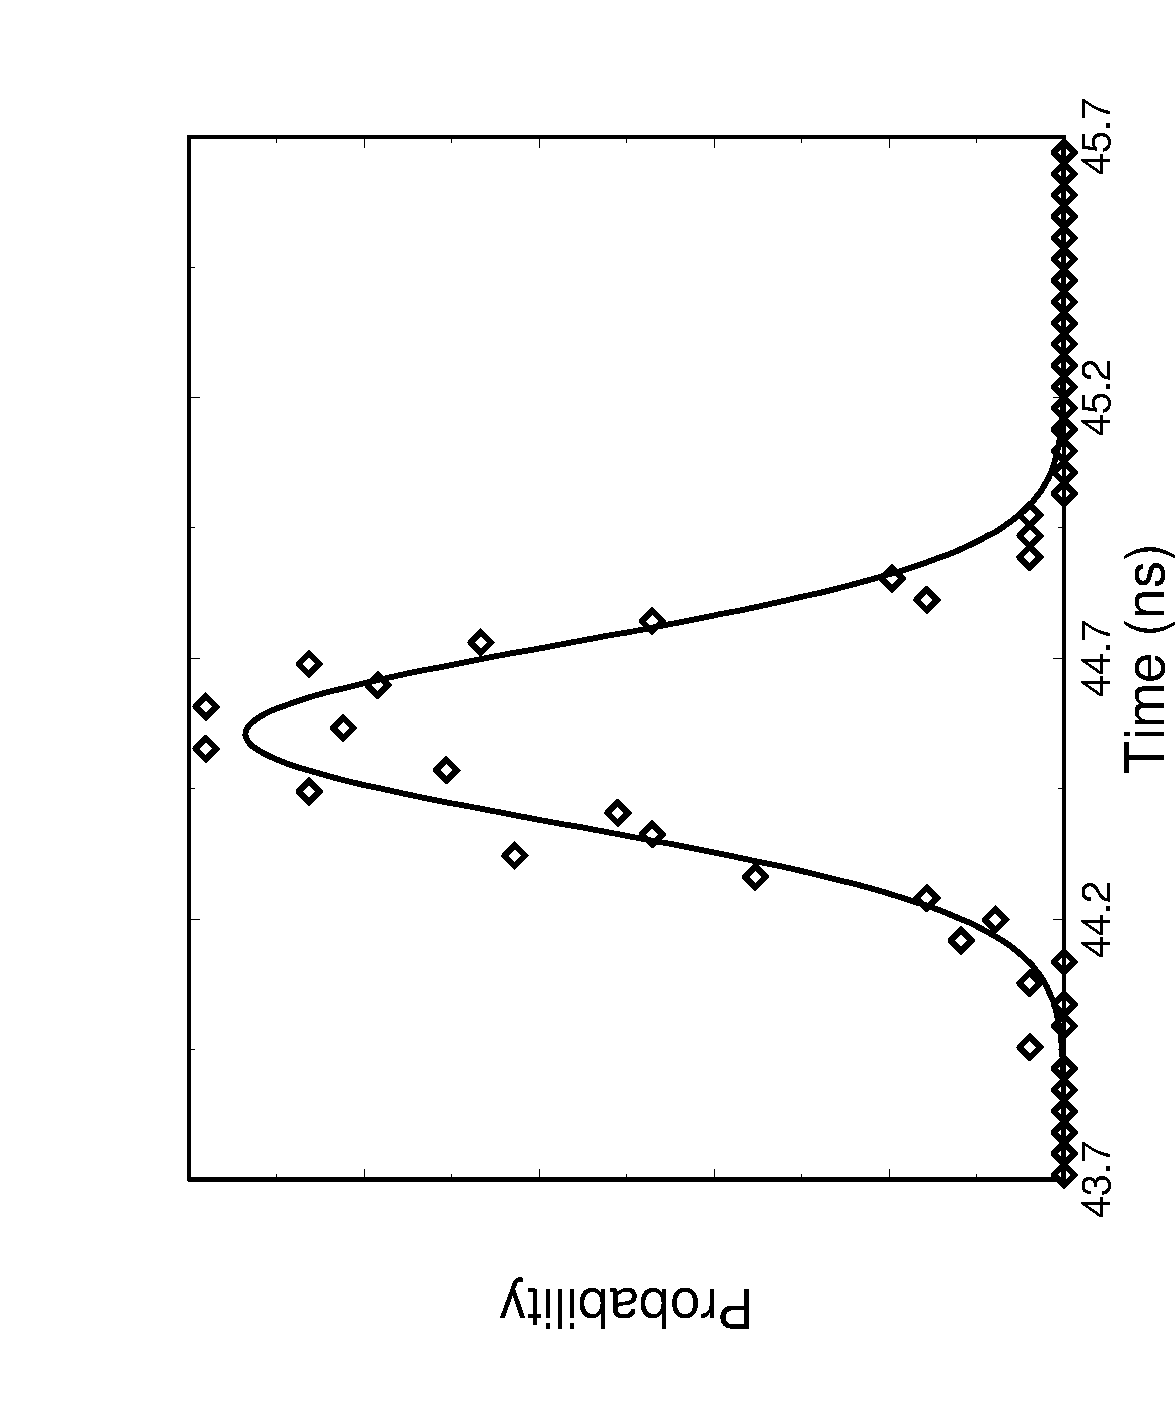
\includegraphics[angle=270, width=4cm]{./graficos/fig_10.pdf}
\caption{Dos gr\'aficos en el mismo entorno.}
\end{figure}
\vspace{-12.5cm}
\begin{figure}[h]
\centerline{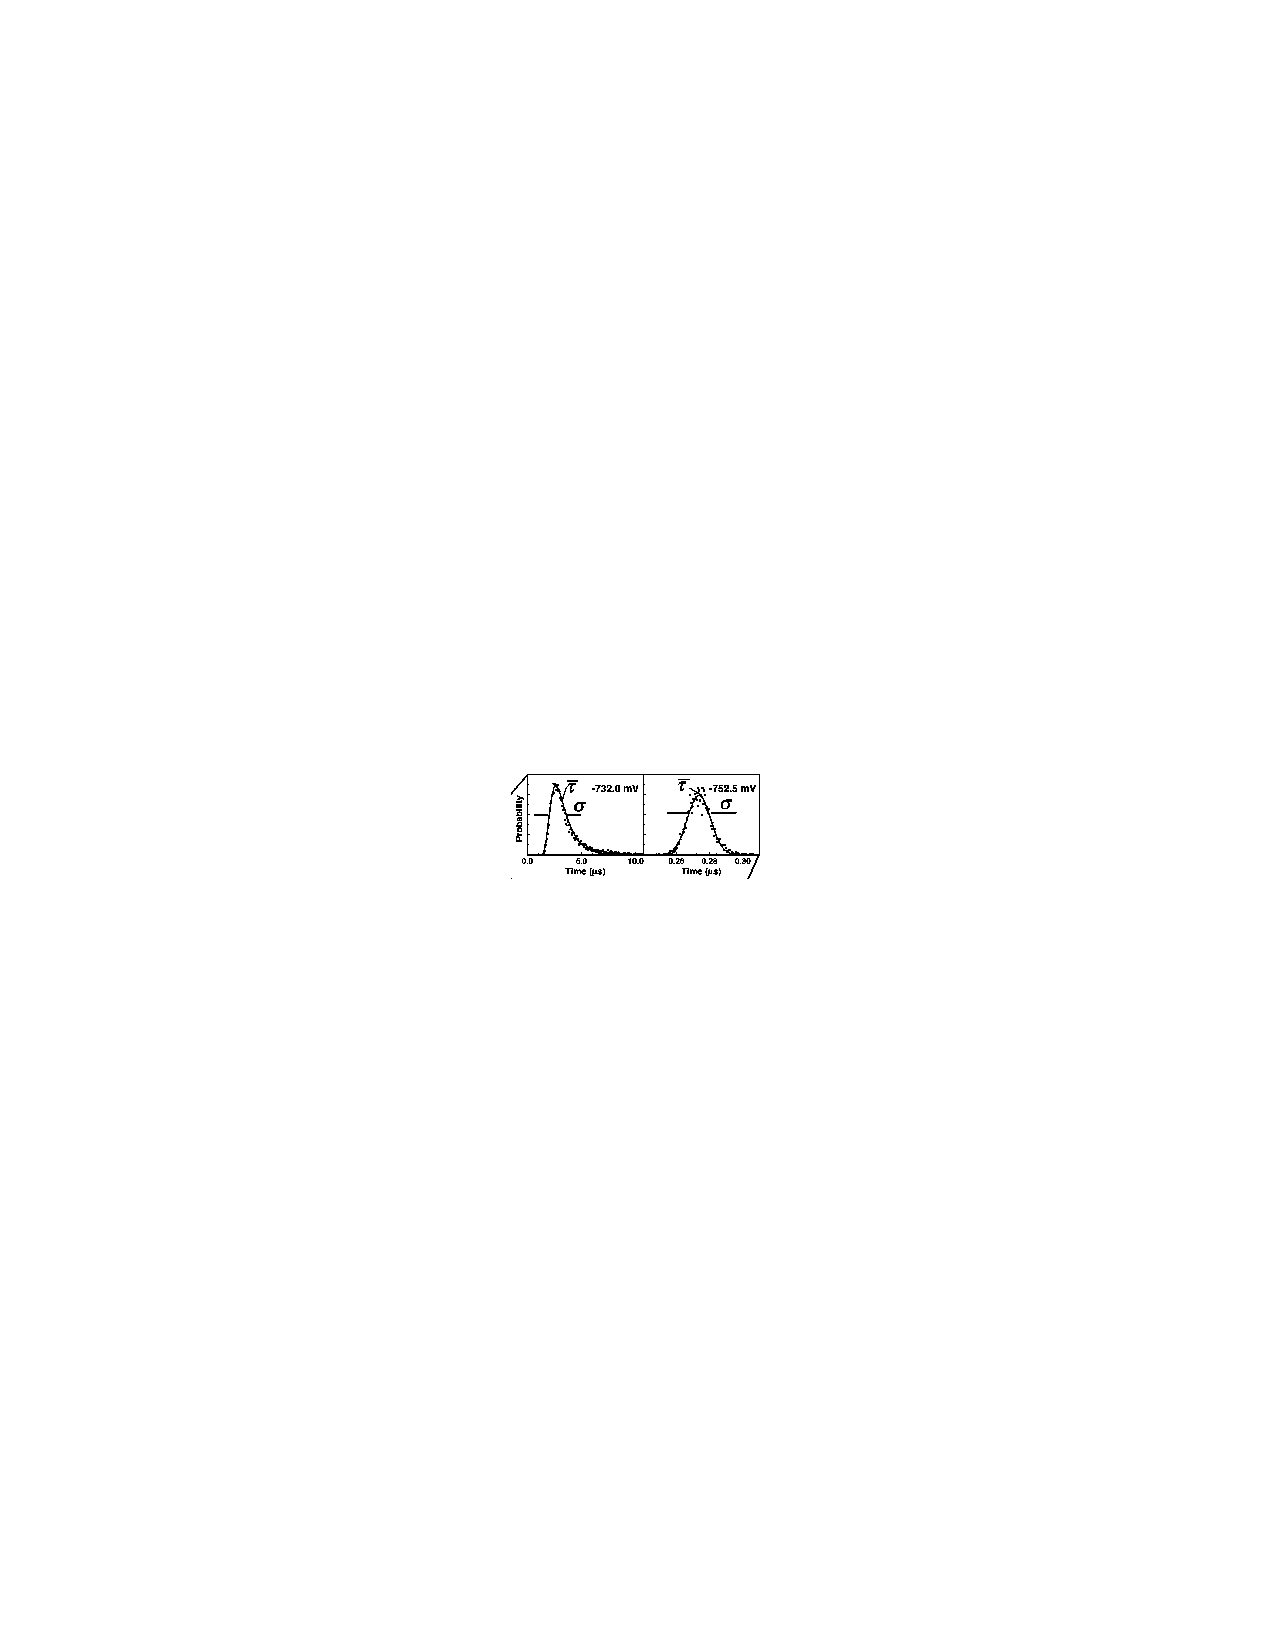
\includegraphics[width=20cm]{./graficos/reloc4.pdf}}
\end{figure}
\end{exampleblock}
\end{frame}

%%%%%%%%%%%%%%%%%%%%%%%%%%%%%%%%%%%%%%%%%%%%%%%%%%%%
\begin{frame}[fragile]
\begin{exampleblock}{Ejercicio 4: Superposici\'on de varios gr\'aficos}
%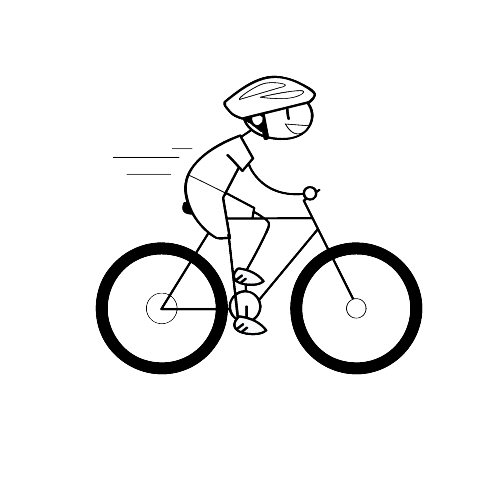
\includegraphics[angle=0, width=3cm]{./graficos/ciclista}
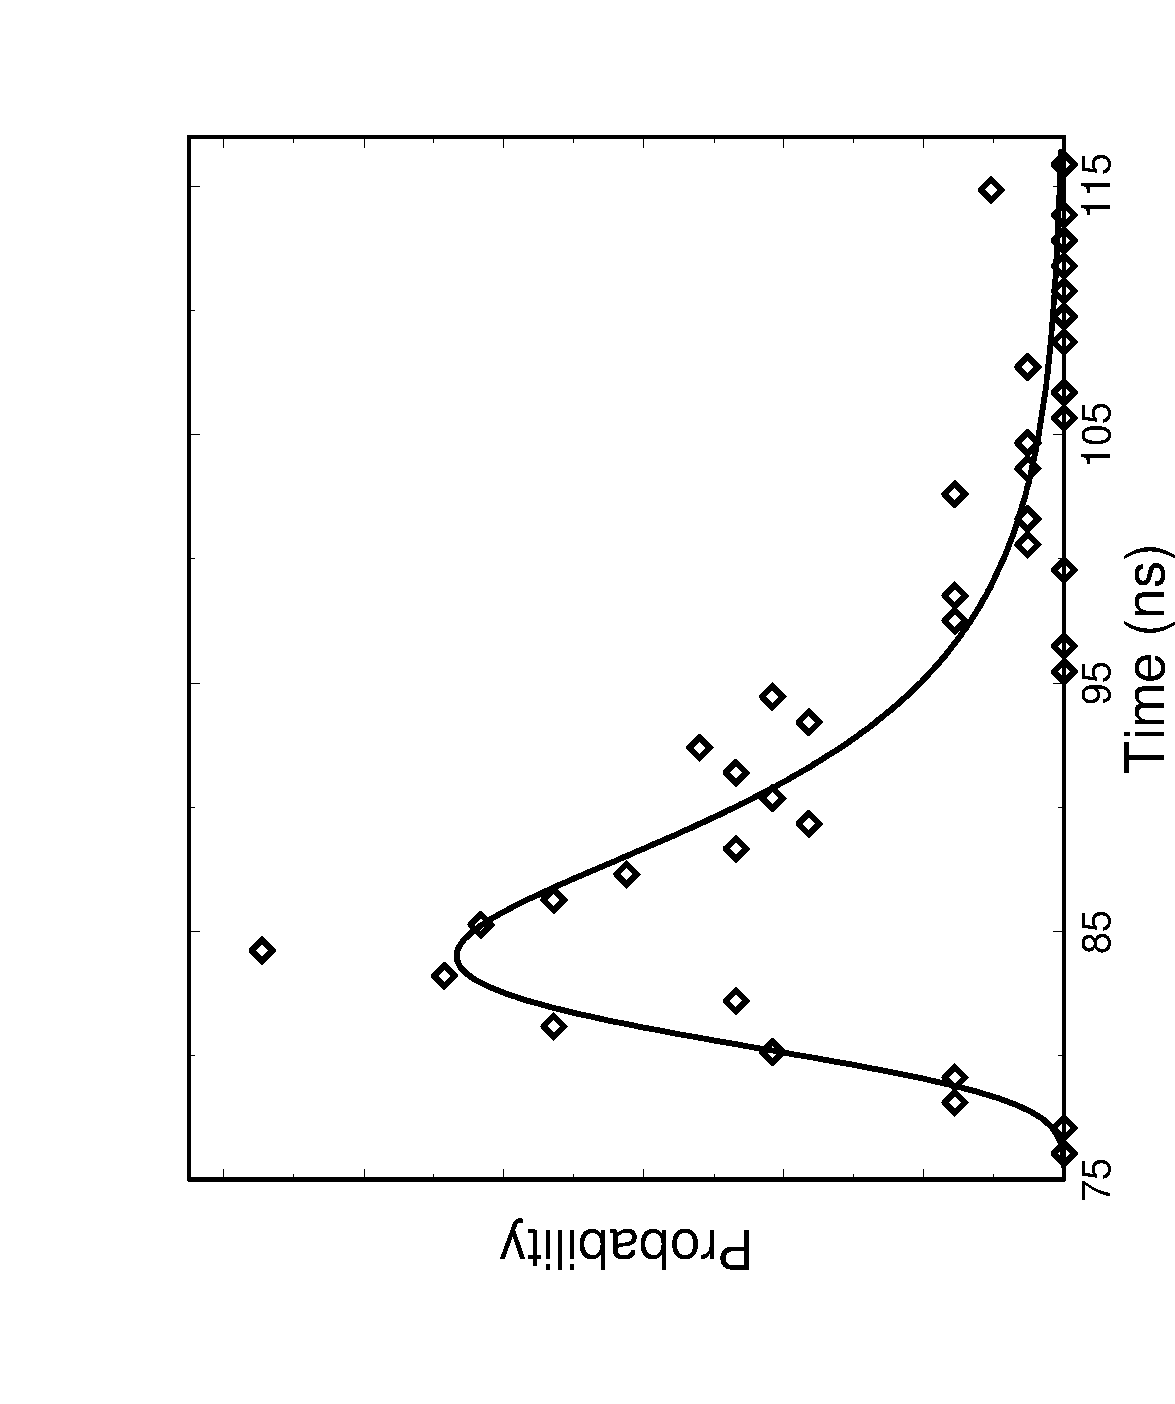
\includegraphics[angle=270,width=9cm]{./graficos/fig_9.pdf}
\put(-100,-205){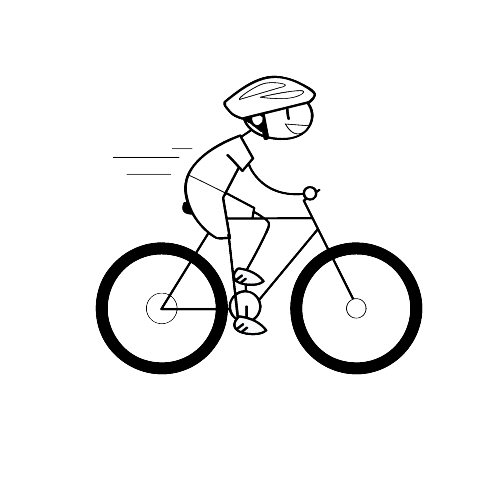
\includegraphics[angle=-7,,scale=0.4]{./graficos/ciclista}}
\end{exampleblock}
\end{frame}


%%%%%%%%%%%%%%%%%%%%%%%%%%%%%%%%%%%%%%%%%%%%%
\section{Creaci\'on de gr\'aficos}
\begin{frame}{Otros paquetes para generar gr\'aficos}
Similarmente, se pueden emplear otros paquetes matem\'aticos 
\begin{enumerate}
\item Mathematica {\small (problemas de fuentes!!!)}
\item Matlab
\item Sage  (Gnuplot)
\item Maxima (Gnuplot)
\item y un largo etc...
\end{enumerate}
Tambien existen paquetes con los que realizar diagramas y representaciones:
\begin{enumerate}
\item \href{http://www.xfig.org}{Xfig} {\small (versi\'on para Windows: WinFIG)}
% Ver Xfig Users's Manual
\item LatexDraw
\item Dia
\item \href{http://www.geogebra.org/cms/}{GeoGebra}
\end{enumerate}
\end{frame}
%%%%%%%%%%%%%%%%%%%%%%%%%%%%%%%%%%%%%%%%%%%%%
\begin{frame}[fragile]{Figura generada con xfig}
\begin{verbatim}
\resizebox{7cm}{!}{\input ./graficos/deformacubos.pdf_t}
\end{verbatim}
\resizebox{7cm}{!}{\input ./graficos/deformacubos.pdf_t}
\end{frame}



%%%%%%%%%%%%%%%%%%%%%%%%%%%%%%%%%%%%%%%%%%%%%
\begin{frame}
\begin{exampleblock}{Ejercicio 3: Generar un gr\'afico con GeoGebra}
\href{http://www.geogebra.org/cms/}{GeoGebra} es un programa especialmente sencillo para
realizar este tipo de gr\'aficos.  Vamos a instalarlo y a jugar un poco.
\definecolor{uququq}{rgb}{0.25,0.25,0.25}
\definecolor{zzttqq}{rgb}{0.6,0.2,0}
\definecolor{qqqqff}{rgb}{0,0,1}
\begin{tikzpicture}[line cap=round,line join=round,>=triangle 45,x=0.7732426303854876cm,y=0.6894409937888198cm]
\draw[->,color=black] (-4.3,0) -- (4.52,0);
\foreach \x in {-4,-3,-2,-1,1,2,3,4}
\draw[shift={(\x,0)},color=black] (0pt,2pt) -- (0pt,-2pt) node[below] {\footnotesize $\x$};
\draw[->,color=black] (0,-3.14) -- (0,3.3);
\foreach \y in {-3,-2,-1,1,2,3}
\draw[shift={(0,\y)},color=black] (2pt,0pt) -- (-2pt,0pt) node[left] {\footnotesize $\y$};
\draw[color=black] (0pt,-10pt) node[right] {\footnotesize $0$};
\clip(-4.3,-3.14) rectangle (4.52,3.3);
\onslide<6->{
  \fill[color=zzttqq,fill=zzttqq,fill opacity=0.1] (-2.16,3.2) -- (0.78,4.52) -- (3,2.68) -- (-1,1) -- cycle;
}
\onslide<6->{
  \draw [color=zzttqq] (0.78,4.52)-- (3,2.68);
}
\onslide<6->{
  \draw [color=zzttqq] (3,2.68)-- (-1,1);
}
\onslide<6->{
  \draw [color=zzttqq] (-1,1)-- (-2.16,3.2);
}
\onslide<7->{
  \draw[smooth,samples=100,domain=-4.3:4.5200000000000005] plot(\x,{sin(((\x))*180/pi)});
}
\onslide<11->{
  \draw [domain=-4.3:4.52] plot(\x,{(-0--1*\x)/1});
}
\onslide<15->{
  \draw(-3.04,4.36) ellipse (0.8cm and 0.71cm);
}
\onslide<16->{
  \draw (4.54,1.96) node[anchor=north west] {$\Sigma_{i=1}^n y_i$};
}
\begin{scriptsize}
\onslide<2->{
  \fill [color=qqqqff] (-2.16,3.2) circle (1.5pt);
}
\onslide<2->{
  \draw[color=qqqqff] (-2,3.46) node {$A$};
}
\onslide<3->{
  \fill [color=qqqqff] (0.78,4.52) circle (1.5pt);
}
\onslide<3->{
  \draw[color=qqqqff] (0.92,4.78) node {$B$};
}
\onslide<4->{
  \fill [color=qqqqff] (3,2.68) circle (1.5pt);
}
\onslide<4->{
  \draw[color=qqqqff] (3.16,2.94) node {$C$};
}
\onslide<5->{
  \fill [color=qqqqff] (-1,1) circle (1.5pt);
}
\onslide<5->{
  \draw[color=qqqqff] (-0.84,1.26) node {$D$};
}
\onslide<8->{
  \fill [color=qqqqff] (5.26,4.04) circle (1.5pt);
}
\onslide<8->{
  \draw[color=qqqqff] (5.4,4.3) node {$E$};
}
\onslide<9->{
  \fill [color=uququq] (0,0) circle (1.5pt);
}
\onslide<9->{
  \draw[color=uququq] (0.14,0.26) node {$F$};
}
\onslide<10->{
  \fill [color=qqqqff] (1,1) circle (1.5pt);
}
\onslide<10->{
  \draw[color=qqqqff] (1.16,1.26) node {$G$};
}
\onslide<12->{
  \fill [color=qqqqff] (-1.18,5.36) circle (1.5pt);
}
\onslide<12->{
  \draw[color=qqqqff] (-1.02,5.62) node {$H$};
}
\onslide<13->{
  \fill [color=qqqqff] (-3.04,4.36) circle (1.5pt);
}
\onslide<13->{
  \draw[color=qqqqff] (-2.94,4.62) node {$I$};
}
\onslide<14->{
  \fill [color=qqqqff] (-2.58,5.28) circle (1.5pt);
}
\onslide<14->{
  \draw[color=qqqqff] (-2.46,5.54) node {$J$};
}
\end{scriptsize}
\end{tikzpicture}

Nota: Es interesante ver las posibilidades que nos ofrece a la hora de exportar el gr\'afico
que acabamos de realizar
\end{exampleblock}
\end{frame}
%%%%%%%%%%%%%%%%%%%%%%%%%%%%%%%%%%%%%%%%%%
\begin{frame}{Gr\'aficos con PSTricks y TikZ}
Tanto \href{http://www.ctan.org/pkg/pstricks}{PSTricks} como \href{http://www.texample.net/tikz/}{PGF-TikZ} son paquetes de LaTeX que permiten crear gr\'aficos mediante comandos espec\'ificos.

Permiten hacer casi cualquier cosa, siempre que estemos dispuestos a invertir nuestro tiempo en ello. Ver manuales, y ejemplos
\begin{itemize}
\item \href{http://www.texample.net/tikz/examples/}{http://www.texample.net/tikz/examples/}
\item \href{http://tug.org/PSTricks/main.cgi?file=examples}{http://tug.org/PSTricks/main.cgi?file=examples}
\end{itemize}

Es por ello que numerosos programas dan la posibilidad de devolver sus gr\'aficos mediante
estos comandos (GeoGebra, LatexDraw, etc....)

{\small Observaciones:
Aunque PSTricks no es compatible con PDFLaTeX, existen versiones (spt-pdf o pdftricks)
que si lo son.}


\end{frame}


%%%%%%%%%%%%%%%%%%%%%%%%%%%%%%%%%%%%%%%%%%%%
\begin{frame}{Ejemplos con TikZ}
\begin{figure}[h]
\begin{center}
\begin{tikzpicture}[>=latex,thick,auto, scale=0.6, transform shape]
\coordinate [label=above:{\bf A)}] (Q) at (-0.5,6.25);
%
\draw[color=black,line width = 1.5pt, domain=5.9:5.5] plot (\x,{2*(6-\x)*exp((-\x+4)/2)});
\draw[color=black,style=dashed,line width = 1pt, domain=5.5:4.75] plot (\x,{2*(6-\x)*exp((-\x+4)/2)});
\coordinate [label=above:{$r$}] (P) at (0,6.5);
\coordinate [label=right:{$u$}] (f) at (6.5,0);
%
\draw[->] (0,0) -- (P) ;
\draw[->] (0,0) -- (f) ;
%
\coordinate [label=below:{$1$}] (f2) at (6,0);
\coordinate [label=left:{$1$}] (P2) at  (0,6);
\fill (6,0) circle (2pt);
\draw[-,style=dashed,dash pattern=on 1pt off 2pt on 1pt off 2pt]
(6,6)-- (P2) ;
\draw[-,style=dashed,dash pattern=on 1pt off 2pt on 1pt off 2pt]
(6,6) -- (f2) ;
%
\coordinate [label=above:{$u^*(\sigma)$}] (u*sigma) at (4,6);
\fill[black] (4,6) circle (2pt);
\coordinate [label=left:{$r^*(\sigma)$}] (r*) at (0,4);
\fill[black] (0,4) circle (2pt);
\draw[arrows = )-angle 60, thin] (1,6)--(0.98,5.5);
\draw[arrows = )-angle 60, thin] (2,6)--(1.91,5.5);
\draw[arrows = )-angle 60,thin] (3,6)--(2.7,5.6);
\draw[arrows = )-angle 60, thin] (4,6)--(3.5,6);
\draw[arrows = )-angle 60, thin] (5,6)--(4.54,6.21);
\draw[arrows = )-angle 60, thin] (6,6)--(5.58,6.27);
\draw[arrows = )-angle 60, thin] (0,6)--(0,5.5);
\draw[arrows = )-angle 60, thin] (0,5)--(0,4.5);
\draw[arrows = )-angle 60, thin] (0,3)--(0,3.5);
\draw[arrows = )-angle 60, thin] (0,2)--(0,2.5);
\draw[arrows = )-angle 60, thin] (0,1)--(0,1.5);
\draw[arrows = )-angle 60, thin] (0,0)--(0,0.5);

\draw[->,thin] (6,1)--(5.54,0.64);
\draw[->,thin] (6,2)--(5.58,1.72);
\draw[->,thin] (6,3)--(5.52,2.84);
\draw[->,thin] (6,4)--(5.5,4);
\draw[->,thin] (6,5)--(5.52,5.15);

\draw[->,thin] (1,0)--(1,0.5);
\draw[->,thin] (2,0)--(2,0.5);
\draw[->,thin] (3,0)--(3,0.5);
\draw[->,thin] (4,0)--(4,0.5);
\draw[->,thin] (5,0)--(5,0.5);

%%% SEGUNDO GRAFICO  %%%%%%%%
\coordinate [label=above:{\bf B)}] (Q) at (7.5,6.25);
\coordinate [label=above:{$r$}] (P) at (8,6.5);
\coordinate [label=right:{$u$}] (f) at (14.5,0);
%
\draw[->] (8,0) -- (P) ;
\draw[->] (8,0) -- (f) ;
%
\coordinate [label=below:{$1$}] (f2) at (14,0);
\coordinate [label=left:{$1$}] (P2) at  (8,6);
%\fill (6,0) circle (2pt);
\draw[-,style=dashed,dash pattern=on 1pt off 2pt on 1pt off 2pt]
(14,6)-- (P2) ;%linea que llega a P2
\draw[-,style=dashed,dash pattern=on 1pt off 2pt on 1pt off 2pt]
(14,6) -- (f2) ;
\draw[solid,line width = 1.5pt] plot file{./graficos/type1Orbit.table};
\coordinate [label=below:{$u^*(\sigma_{smooth})$}] (u*sigsmooth) at (9.96078080000047,0);
\draw[-,style=dotted,line width = 0.5pt] (9.96078080000047,0) --  (9.96078080000047,6.001506405627179);
\fill[black] (9.96078080000047,6.001506405627179) circle (2.5pt);
\coordinate [label=above:{$u^*(\sigma_{ent})$}] (u*sigsmooth) at (11.001864692901634,5.99984352366344);
\fill[black] (10.501864692901634,5.99984352366344) circle (2.5pt);
\end{tikzpicture}
\end{center}
\caption{{A)} Normalized direction field {B)} Numerical solutions to Type I (solid), II (dashed) and III (dotted) orbits .
}
\label{orbitas}
\end{figure}

\end{frame}
%%%%%%%%%%%%%%%%%%%%%%%%%%%%%%%%%%%%%%%%%%%%
\begin{frame} {Ejemplo con TikZ}
No hay que pensar que \'unicamente podemos hacer gr\'aficos. 
Estas herramientas nos dan mucho juego a la hora de hacer por ejemplo 
presentaciones.

\begin{tikzpicture}[]
%% Draw events and edges

%% Draw system flow diagram
  \begin{scope}[xshift=-7.5cm,yshift=-5cm,very thick,
       node distance=1.4cm,on grid,>=stealth',
       caja/.style={rectangle,draw,fill=red!90},
       redondel/.style={circle,draw,fill=blue!70},]
   \node [redondel] (meritos)  {$\begin{array}{c}\mbox{T\'{\i}tulo y}\\ \mbox{expediente}\end{array}$};
     % \node [caja] (titulo)         [above=of meritos] {$\begin{array}{c}\mbox{T\'{\i}tulo}\\ \mbox{Grado}\end{array}$};
    \node [redondel] (pregunta)    [right =of meritos,xshift=1cm]{?};
    \draw[->] (meritos) -- (pregunta);
    \node [redondel] (pregunta3)    [right =of pregunta,yshift=-1.0cm,xshift=0.5cm]{\footnotesize  Inquietud};
    \node [redondel] (pregunta2)    [right =of pregunta,xshift=0.5cm]{\footnotesize Vocaci\'on};
    \node [redondel] (pregunta1)    [right =of pregunta,yshift=1.0cm,xshift=0.5cm]{\ \ \ $\$ \$$ \ \ \ };
   \draw[->] (pregunta) -- (pregunta3);
   \draw[->] (pregunta) -- (pregunta2);
   \draw[->] (pregunta) -- (pregunta1);
    \node [caja] (inves)  [right =of pregunta3,xshift=2.0cm]{Investigaci\'on};
    \node [caja] (docen) [right =of pregunta2,xshift=2.0cm] {Docencia};
   \node [caja] (word)    [right =of pregunta1,xshift=2.0cm] {Mundo laboral};
   %\draw[->] (pregunta1) -- (inves);
   \draw[->] (pregunta1) -- (docen);
   \draw[->] (pregunta1) -- (word);
   \draw[->] (pregunta2) -- (inves);
   \draw[->] (pregunta2) -- (docen);
   \draw[->] (pregunta2) -- (word);
   \draw[->] (pregunta3) -- (inves);
   %\draw[->] (pregunta3) -- (docen);
   %\draw[->] (pregunta3) -- (word);
   %\draw[->] (inves) -- (docen);
%    \node [redondel] (pregunta)    [left =of docen,yshift=-0.0cm]{?} edge [->] (inves) edge [->] (docen) edge [->] (word);
%    \node [caja] (inves)  {(vocacional) Investigaci\'on};
%   \node [caja] (meritos)  {$\begin{array}{c}\mbox{A\~nos}\\ \mbox{expediente}\end{array}$};
%    \node [caja] (titulo)         [above=of meritos] {$\begin{array}{c}\mbox{T\'{\i}tulo}\\ \mbox{Grado}\end{array}$} edge [<->] (meritos);
       \end{scope}
\end{tikzpicture}
\end{frame}




%%%%%%%%%%%%%%%%%%%%%%%%%%%%%%%%%%%%%%%%%%%%
\begin{frame}[fragile]{Bibliograf\'ia}
\begin{thebibliography}{10}
\bibitem{ManualLatexWikilibros} \href{http://es.wikibooks.org/wiki/Manual_de_LaTeX/Insertar_figuras_en_un_documento}{Manual de Latex/ Insertar figuras en un documento- Wikilibros.}

\bibitem{ManualImportingGraphics}\href{http://en.wikibooks.org/wiki/LaTeX/Importing_Graphics}{Latex/Importing Graphics-Wikilibros.}

\bibitem{wrapfigure} \href{http://www.ctan.org/pkg/wrapfig}{P\'agina del paquete wrapfig, ctang.org}

\end{thebibliography}
\end{frame}




\end{document}